\chapter{简单系统的热力学性质}
\label{chap:simple system}

\section{形式关系}

\begin{definition}
	{广延量和强度量}{extensive parameter & intensive parameter}
	内能$U$、体积$V$、熵$S$和摩尔数$n$等物理量,系统的量等于子系统的量之和,称为广延量(extensive parameter):
	\begin{equation}
		S(U,V,n)=\sum_{i=1}^kS_i(U_i,V_i,n_i).
	\end{equation}
	而温度$T$、压强$p$%和化学势$\mu$
	等物理量与广延量的比值有关,平衡时各子系统的量相同,称为强度量(intensive parameter)。
\end{definition}

\begin{theorem}
	{Euler方程}{Euler's equation}
	若$r$元函数$f$满足$k$阶齐次条件,即$\forall\lambda\geq 0$均有
	\begin{equation}
		\label{eq:k-order homogeneous}
		f(\lambda x_1,\lambda x_2,\ldots,\lambda x_r)=\lambda^k f(x_1,x_2,\ldots,x_r),
	\end{equation}
	则应有
	\begin{equation}
		\label{eq:Euler's equation}
		f(x_1,x_2,\ldots,x_r)=\frac1k\sum_{i=1}^r x_i\pv f{x_i}.
	\end{equation}
\end{theorem}

\begin{proof}
	对\eqref{eq:k-order homogeneous}两边同时对$\lambda$求导
	\[
		x_1\pv f{\lambda x_1}+x_2\pv f{\lambda x_2}+\cdots+x_r\pv f{\lambda x_r}=k\lambda^{k-1}f(x_1,x_2,\ldots,x_r).
	\]
	取$\lambda=1$即得\eqref{eq:Euler's equation}。
\end{proof}

\begin{corollary}
	广延量$U=U(S,V)$是一阶齐次的,故
	\begin{equation}
		\label{eq:U=TS-pV}
		U=TS-pV.
	\end{equation}
	由此可定义单位摩尔的内能$u:=U/n$、熵$s:=S/n$和体积$v:=V/n$,以及热容$c:=C/n$。
\end{corollary}

\begin{theorem}
	{Gibbs-Duhem关系}{Gibbs-Duhem relation}
	$S$和$V$的约束关系为:
	\begin{equation}
		S\d T-V\d p=0.
	\end{equation}
\end{theorem}

\begin{proof}
	对\eqref{eq:U=TS-pV}两边微分,再结合\eqref{eq:dU=TdS-pdV}消去一些项即得
	\[
		\cancel{\d U}=\cancel{T\d S}+S\d T\,\cancel{-p\d V}-V\d p.
		\qedhere
	\]
\end{proof}

\begin{example}{用形式关系求基本方程}{}
	某热力学系统的内能和状态方程为
	\[
		U=\frac12pV,\qquad T^2=A\frac{U^{3/2}}{Vn^{1/2}}.
	\]
	其中常数$A>0$,求系统的基本方程。

	条件中出现的广延量为$U,V,n$,因此用熵表象,考虑单位摩尔熵$s=s(u,v)$
	\begin{align*}
		\frac1T&=A^{-1/2}u^{-3/4}v^{1/2},\\
		\frac pT&=2A^{-1/2}u^{1/4}v^{-1/2}.
	\end{align*}
	凑微分:
	\begin{gather*}
		\d s=\frac1T\d u+\frac pT\d v=A^{-1/2}(u^{-3/4}v^{1/2}\d u+2u^{1/4}v^{-1/2}\d v)=4A^{-1/2}\d(v^{1/4}u^{1/2}),\\
		\implies
		s=4A^{-1/2}u^{1/4}v^{1/2}+s_0,
	\end{gather*}
	即
	\[
		S=4A^{-1/2}U^{1/4}V^{1/2}n^{1/4}+ns_0.
	\]
\end{example}

\section{热力学其他表象}

在能量表象和熵表象中,广延量是数学上的独立变量,而强度量是被导出的物理量;%这与现实中实验操作的便利性截然不同。
然而,有时强度量更容易测量或控制,
最突出的是熵$S$和温度$T$这一对共轭变量:并不存在可以测量和控制熵的仪器,而温度计和恒温器在实验室中十分常见。
这种情况下更适合将强度量作为独立变量,广延量作为导出量。
这就需要Legendre变换。
% 这样还能够导出很多其它的热力学表象。


\begin{theorem}
	{Legendre变换}{Legendre transformation}
	考虑函数$y=y(x)$,其在$x$处的切线斜率为$p$、纵截距为$\psi$,则存在$(x,y)\mapsto(p,\psi)$:
	\begin{subequations}
		\label{eq:Legendre transformation}
		\begin{align}
			p&=\dv yx,\\
			\psi&=y-px,
		\end{align}
	\end{subequations}
	称为Legendre变换。
	\begin{center}
		\includegraphics[page=6]{figures/tikz/coordinates.pdf}
		\captionof{figure}{Legendre变换}
		\label{fig:Legendre transform}
	\end{center}
\end{theorem}

\begin{corollary}
	为了满足变换的可逆性,要求$p=y'$严格单调(即$y$具有凹凸性),从而
	\[
		\d\psi=\d y-(p\d x+x\d p)=-x\d p,
	\]
	可得Legendre逆变换
	\begin{subequations}
		\begin{align}
			x&=-\dv\psi p,\\
			y&=\psi+px.
		\end{align}
	\end{subequations}
\end{corollary}

\begin{corollary}
	推广到多元函数$y(x_1,x_2,\ldots,x_r)$,其Legendre变换为
	\[
		\begin{aligned}
			p_i  & =\pv y{x_i}            \\
			\psi & =y-\sum_{i=1}^rp_ix_i.
		\end{aligned}
		\iff
		\begin{aligned}
			x_i & =-\pv\psi{p_i}            \\
			y   & =\psi+\sum_{i=1}^rp_ix_i.
		\end{aligned}
	\]
\end{corollary}

\begin{example}{分析力学中的Legendre变换}{}
	Lagrange量$L(q,\dot q,t)$可以完整刻画一个力学系统,
	其中$q=(q_1,q_2,\ldots,q_r)$为广义坐标,$\dot q=(\dot q_1,\dot q_2,\ldots,\dot q_r)$为广义速度。广义动量定义为
	\[
		p_i:=\pv L{\dot q_i}.
	\]
	如果以动量代替速度作为独立变量,则需要对$\dot q_i$做Legendre变换,引入Hamilton量
	\begin{equation}
		H(q,p,t):=\sum_{i=1}^rp_i\dot q_i-L(q,\dot q,t).
	\end{equation}
	这样$H(q,p,t)$关于广义动量$p_i$的导数便是广义速度
	\[
		\pv H{p_i}=\dot q_i.
	\]
\end{example}

从已有的能量$U=U(S,V)$出发,进行一系列Legendre变换,得到其它热力学表象。
% 从能量$\d U=T\d S-p\d V$出发

\begin{definition}
	{焓}{enthalpy}
	考虑等压过程,$V\to p=-\p U/\p V$,可得焓(enthalpy) $H=H(S,p)$
	\begin{subequations}
		\begin{align}
			H&=U+pV,\\
			\d H&=T\d S+V\d p.
		\end{align}
	\end{subequations}
	% \begin{equation}
	% 	H=U+pV.
	% \end{equation}
\end{definition}

\begin{definition}
	{Helmholtz自由能}{Helmholtz free energy}
	考虑等温过程,$S\to T=\p U/\p S$,可得Hemholtz自由能$F=F(T,V)$
	\begin{subequations}
		\begin{align}
			F&=U-TS,\\
			\d F&=-S\d T-p\d V.
		\end{align}
	\end{subequations}
	% \begin{equation}
	% 	F=U-TS.
	% \end{equation}
\end{definition}

\begin{corollary}
	自发的等温等容过程中$\D F=\D U-T\D S=Q-T\D S\leq 0$自由能减少。
\end{corollary}

\begin{definition}
	{Gibbs自由能}{Gibbs free energy}
	考虑等温等压过程,$(S,V)\to(T,p)$,可得Gibbs自由能$G=G(T,p)$
	\begin{subequations}
		\begin{align}
			G&=U-TS+pV,\\
			\d G&=-S\d T+V\d p.
		\end{align}
	\end{subequations}
	% \begin{equation}
	% 	G=U-TS+pV.
	% \end{equation}
\end{definition}

\begin{corollary}
	自发的等温等压过程中$\D G=\D U-T\D S+p\D V=Q-T\D S\leq 0$自由能减少。
\end{corollary}

\begin{definition}{特性函数}{characterist funtion}
	适当选取自变量,只需一个热力学量就可决定均匀系统的全部热力学性质,这样的函数称为特性函数(characterist funtion)。
	包括$U(S,V),H(S,p),F(T,V),G(T,p)$等。
\end{definition}

\begin{theorem}
	{Maxwell关系}{Maxwell relation}
	由特性函数$U(S,V),F(T,V),H(S,p),G(T,p)$的二阶导可交换:
	\begin{subequations}
		\begin{alignat}{3}
			\label{eq:Maxwell relation U}
			\pw USV&=\pw UVS&&\implies& -\pu[V]pS&=\pu[S]TV;\\
			\label{eq:Maxwell relation H}
			\pw HSp&=\pw HpS&&\implies& \pu[p]VS&=\pu[S]Tp;\\
			\label{eq:Maxwell relation F}
			\pw FTV&=\pw FVT&&\implies& \pu[V]pT&=\pu[T]SV;\\
			\label{eq:Maxwell relation G}
			\pw GTp&=\pw GpT&&\implies& -\pu[p]VT&=\pu[T]Sp.
		\end{alignat}
	\end{subequations}
	称为Maxwell关系。
	可以借助图形记忆,如\figref{fig:Maxwell relation} 所示,
	外围方形四边上的$U,F,H,G$是四个特性函数,每边的两个顶点分别是状态参量,如$U(S,V)$,对角线连接状态参量和导出量,箭头方向表示正负号,如$\d U=T\d S-p\d V$。再由二阶导可交换便可得到Maxwell关系。
	至于\figref{fig:Maxwell relation} 中字母的顺序,则可以通过一句口诀中的首字母记忆。
	\footnote{其实还不如直接记住$\d U=T\d S-p\d V$和$H=U+pV$,剩下的其实很自然得都出来了。}
	\begin{center}
		\includegraphics[page=3]{figures/tikz/layouts.pdf}
		\captionof{figure}{\textbf{G}ood \textbf{p}hysicists \textbf{H}ave \textbf{S}tudied \textbf{U}nder \textbf{V}ery \textbf{F}ine \textbf{T}eachers.}
		\label{fig:Maxwell relation}
	\end{center}
\end{theorem}

\begin{corollary}
	考虑Gibbs自由能$G(T,p)$的二阶导:
	\begin{subequations}
		\begin{alignat}{2}
			\pv[2]GT&=-&\pu[p]ST&=-\frac{C_p}T,\\
			\pw GTp&=&\pu[p]VT&=V\alpha,\\
			\pv[2]Gp&=&\pu[T]Vp&=-V\kappa_T.
		\end{alignat}
	\end{subequations}
	因此难以直接测量的响应函数(热力学偏微分)都可以用$C_p,\alpha,\kappa_T$来表示。
\end{corollary}

\begin{example}
	{热弹效应}{}
	由Maxwell关系
	\[
		\pu[T]Sp=-\pu[p]VT=-V\alpha.
	\]
	说明弹性材料在伸长(或缩短)时会放热(或吸热),而且其熵变大小与形变量有关。
\end{example}

\begin{example}
	{热容差}{}
	由于液体一般很难压缩,等容热容$C_V$相比等压热容$C_p$更难测量,但是我们可以将二者的差用$\alpha,\kappa_T$表示出来。
	继续\exmref{exm:ideal gas U and C} 的推导。
	利用Maxwell关系\eqref{eq:Maxwell relation F},
	\[
		C_p-C_V=\biggfkh{\pu[T]UV+p}\pu[p]VT=T\pu[T]SV\pu[p]VT=-T\pu[V]pT\pu[p]VT.
	\]
	代入响应函数可得
	\begin{equation}
		C_p-C_V=-pVT\alpha\beta=\frac{VT\alpha^2}{\kappa_T}.
	\end{equation}
	\tcblower
	类似地,可定义绝热压缩率
	\begin{equation}
		\kappa_S:=-\frac1V\pu[S]Vp,
	\end{equation}
	压缩率的差也存在类似的关系,自证不难
	\begin{equation}
		\kappa_T-\kappa_S=\frac{VT\alpha^2}{C_p}.
	\end{equation}
\end{example}

\begin{example}{}{}
	化简$\pu[G]pU=\pu[G]Up^{-1}$,由$\d U=T\d S-p\d V$可得
	\[
		\pu[G]Up=T\pu[G]Sp-p\pu[G]Vp,
	\]
	利用\eqref{eq:XY->XW/YW}和$\d G=-S\d T+V\d p$可得
	\[
		\pu[G]Up=-T\fracdisp{\pu[S]Gp}{\pu[p]GS}+p\fracdisp{\pu[V]Gp}{\pu[p]GV}=-T\fracdisp{-S\pu[S]Tp+V}{-S\pu[p]TS+0}+p\fracdisp{-S\pu[V]Tp+V}{-S\pu[p]TV+0}.
	\]
	由响应函数的定义、\eqref{eq:XY->XW/YW}和Maxwell关系
	\begin{align*}
		\pu[p]TV&=\frac1{V\alpha},\\
		\pu[p]TS&=\frac{T}{C_p},\\
		\pu[S]Tp&=-\division{\pu[T]Sp}{\pu[p]ST}=\frac{TV\alpha}{c_p},\\
		\pu[V]Tp&=-\division{\pu[T]Vp}{\pu[p]VT}=\frac{\kappa_T}\alpha.
	\end{align*}
	故
	\[
		\pu[G]pU=\biggkh{-TV\alpha+\frac{VC_P}S+PV\kappa_T-\frac{PV^2\alpha}S}^{-1}.
	\]
\end{example}

\section{最值原理}

物理系统有使熵变大的倾向,这一过程会释放能量。可以利用这一性质来做功。

\begin{theorem}
	{最大功原理}{maximum work principle}
	当系统的初末态确定时,可逆过程做功最大。
\end{theorem}

\newcommand{\rev}{_{\mathrm r}}

\begin{proof}
	用可逆功源接受功$\d W\rev$,用可逆热源吸热$\d Q\rev$,下标表示可逆过程。
	能量守恒要求
	\[
		\vd Q+\vd W+\d Q\rev+\d W\rev=0.
	\]
	熵增原理要求
	\[
		\d S+\frac{\d Q\rev}{T\rev}\geq 0.
	\]
	因此
	\[
		\d W\rev\leqslant T\rev\d S-\vd Q-\vd W=\biggkh{1-\frac{T\rev}{T}}(-\vd Q)+(-\vd W).
	\]
	当且仅当熵不变,可逆功取到最大值。
\end{proof}

\begin{corollary}
	对于一个与热库接触的系统,可逆过程所做的功等于Helmholtz自由能的减少量:
	\[
		\d W=-\d(U+U\rev)=-\d(U-T\rev S)=-\d F.
	\]
	自由能的名字正代表\textit{一定条件下可获得的功}。
\end{corollary}

\begin{example}{}{}
	两个等容等摩尔的理想气体通过热机连接,温度分别为$T_1,T_2$,求热机所能输出最大功。

	平衡态两系统温度相等$T$,则能量变化
	\[
		\D U=cnR(2T-T_1-T_2).
	\]
	为使功最大,应为可逆过程,即
	\[
		\D S=cnR\biggkh{\ln\frac T{T_1}+\ln\frac T{T_2}}=cnR\ln\biggkh{\frac{T^2}{T_1T_2}}=0
		\implies T=\sqrt{T_1T_2}.
	\]
	最大功为
	\[
		W=-\D U=cnR\Bigkh{\sqrt{T_1}-\sqrt{T_2}}^2.
	\]
\end{example}
\begin{example}{}{}
	三个等容等摩尔的理想气体通过热机连接,温度分别为$T_1,T_2,T_3$,求其中一个所能达到的最大温度。

	需要热机在两个温度间运行做最大功,将能量传递给第三个系统。最终最高温度系统的温度是$T\hi$,另两个系统的温度均为$T\lo$。由能量守恒,
	\[
		T\hi+2T\lo=T_1+T_2+T_3=:T\tot.
	\]
	总熵变
	\[
		\D S=cnR\ln\biggkh{\frac{T\lo^2T\hi}{T_1T_2T_3}}\geq 0
		\implies(T\tot-T\hi)^2T\hi\geq 4T_1T_2T_3.
	\]
	阴影部分便对应满足条件的$T\hi$的范围(显然,阴影部分总是存在的),
	进而可得到其最大值$T\maxi$。
	\begin{center}
		\includegraphics[page=7]{figures/tikz/coordinates.pdf}
		\captionof{figure}{$T\hi$满足的条件}
	\end{center}
\end{example}

\begin{theorem}
	{能量最小原理}{minimum energy principle}
	在总的熵确定时,任何不受约束的内部参量在平衡时的取值都使得能量最小。
\end{theorem}

\begin{proof}
	根据熵最大原理:在总的内部能量确定时,任何不受约束的内部参量在平衡时的取值都使得熵最大。
	\[
		\pu[U]SX=0,\quad\biggkh{\pv[2]SX}_U<0.
	\]
	其中$X$表示其他状态参量。
	为方便,记能量的一阶导
	\[
		L:=\pu[S]UX=-\division{\pu[U]SX}{\pu[X]SU}=-T\pu[U]SX=0.
	\]
	再证能量的二阶导为正
	\[
		\biggkh{\pv[2]UX}_S=\pu[S]LX=\pu[X]LU\cancel{\pu[S]UX}+\pu[U]LX=0-T\biggkh{\pv[2]SX}_U>0.
		\qedhere
	\]
\end{proof}

\begin{theorem}
	{Helmholtz自由能最小原理}{}
	与恒温热库$T\rev$接触的系统,移除内部约束后达到平衡态使得Helmholtz自由能最小。
	%平衡态下,系统与热库进行热接触	时,系统的各个无约束的内部参量取值满足在 T = Tr 的条件下最小化 Helmholtz 自由能。
\end{theorem}

\begin{proof}
	热库是恒温$T\rev$的,平衡时系统与热库总能量最小,一阶导
	\[
		\d(U+U\rev)=\d U+T\rev\d S\rev=\d U-T\rev\d S\equiv\d F=0.
	\]
	二阶导
	\[
		\d^2(U+U\rev)=\d^2(U-T\rev S\rev)\equiv\d^2F>0.\qedhere
	\]
	
\end{proof}

\begin{corollary}
	平衡态的限制条件为$T=T\rev$。
	当这个系统被活塞隔开时
	\[
		\d F=\pv F{V_1}\d V_1+\pv F{V_2}\d V_2=(-p_1+p_2)\d V_1=0.
	\]
	因此平衡时$p_1=p_2.$
\end{corollary}

\begin{theorem}
	{焓最小原理}{}
	与压强库接触的系统,保持熵不变,移除内部约束后达到平衡态使得焓最小。
\end{theorem}

\begin{theorem}
	{Gibbs自由能最小原理}{}
	与恒温恒压库接触的系统,移除内部约束后达到平衡态使得Gibbs自由能最小。
\end{theorem}

\section{稳定性}

已经提到,$S=S(U,V)$应该是严格上凸的:
\begin{equation}
	\pv[2]SU\pv[2]SV>\biggkh{\pw SUV}^2>0.
\end{equation}

\section{样例系统}

\subsection{理想气体}

前面已经给过,在一定温度范围内,
理想气体内能和状态方程为
\begin{subequations}
	\begin{align}
		u&=cRT,\\
		pv&=RT.
	\end{align}
\end{subequations}
% 其中$c$与理想气体自由度有关,$R=\NA\kB=\SI{8.3144}{\joule\per\mole\kelvin}$是普适的理想气体常数。
% \footnote{最新的国际制基本单位\textit{定义}Avogadro常数$\NA\equiv\SI{6.02214076e23}{\per\mole}$;Boltzmann常数$\kB\equiv\SI{1.380649e-23}{\joule\per\kelvin}$,因此理想气体常数也是精确的。}
可以直接得到响应函数
\begin{subequations}
	\begin{align}
		c_V&=\pu[V]uT=\frac uT=cR,\\
		c_p&=\pu[p]uT+p\pu[p]vT=(c+1)R,\\
		\alpha&=\frac1v\pu[p]vT=\frac1T,\\
		\beta&=-\frac1p\pu[v]pT=-\frac1T,\\
		\kappa_T&=-\frac1v\pu[T]vp=\frac1p.
	\end{align}
\end{subequations}
选定参考点$s_0=s(u_0,v_0)$后,摩尔熵$s$的表达式为
\begin{equation}
	s=R\ln\biggfkh{\biggkh{\frac u{u_0}}^c\frac v{v_0}}+s_0.
\end{equation}
摩尔Helmholtz自由能$f=u-Ts$是$T,v$的函数,写成更简洁的形式:
\begin{equation}
	\frac fT=-R\ln\biggfkh{\biggkh{\frac T{T_0}}^c\frac v{v_0}}+\frac{f_0}{T_0}.
\end{equation}
Gibbs自由能$g=u-Ts+pv$是$T,p$的函数:
\begin{equation}
	\frac gT=-R\ln\biggfkh{\biggkh{\frac T{T_0}}^{c+1}\frac{p_0}p}+\frac{g_0}{T_0}.
\end{equation}
% 考虑等温过程,$\D G=nRT\ln(p'/p)$,这一简单关系在\chapref{chap:phase}中会被用到。

\subsectionstar{van der Waals气体}

在低温、高压的条件下,理想气体就与实际气体相差较远了。
van der Waals气体是对理想气体的一个比较好的修正:
考虑理想气体的摩尔熵$s=R\ln(u^cv)+\const$,将其中的摩尔内能$u$减去分子间平均吸引势能$-a/v$,并将摩尔体积$v$减去分子的体积效应$b$,得到
\begin{equation}
	s=R\ln\Bigfkh{\Bigkh{u+\frac av}^c(v-b)}+\const.
\end{equation}
由此可得到van der Waals气体的内能和状态方程:
\begin{subequations}
	\begin{gather}
		u=cRT-\frac av,\\
		\Bigkh{p+\frac a{v^2}}(v-b)=RT.
	\end{gather}
\end{subequations}
进而得到响应函数
\begin{subequations}
	\begin{align}
		c_V&=cR,\\
		c_p&=\biggkh{c+\frac{RTv^3}{RTv^3-2a(v-b)^2}}R>(c+1)R,\\
		\alpha&=\frac{Rv^2(v-b)}{RTv^3-2a(v-b)^2},\\
		\kappa_T&=\frac{v^2(v-b)^2}{RTv^3-2a(v-b)^2}.
	\end{align}
\end{subequations}
在低密度极限$v\to\infty$下,形式变成$pv=RT$,$\alpha=1/T$,$\kappa_T=v/RT=1/p$,变成理想气体情形。

\subsectionstar{黑体辐射}

在一个黑体辐射系统中,内能和状态方程为
\begin{subequations}
	\begin{align}
		U&=\frac{4\sigma}cVT^4,\\
		p&=\frac13\frac UV=\frac{4\sigma}{3c}T^4.
	\end{align}
\end{subequations}
其中$\sigma$是Stefan-Boltzmann常数,$c$在这里是光速。

可得相应函数(恒压过程同时也为恒温过程,$C_p,\alpha,\kappa_T$无意义):
\begin{subequations}
	\begin{align}
		C_V&=\pu[V]UT=4\frac UT=\frac{16\sigma}cVT^3,\\
		\beta&=-\frac1p\pu[V]pT=-\frac4T.
	\end{align}
\end{subequations}
熵的微分$\d S=(\d U+p\d V)/T$,积分可得熵
\begin{equation}
	S=\frac43\frac UT=\frac{16\sigma}{3c}VT^3.
\end{equation}
因此绝热过程满足$VT^3=\const$;
Gibbs自由能
\begin{equation}
	G=U-TS+pV=0.
\end{equation}

\subsection{电介质和磁介质}

\paragraph{电介质}

电偶极矩为$\bm p_\elc$的电介质放入电场$\bm E$中,Gibbs自由能
\[
	\d G=-S\d T+V\d p-p_\elc\d E
\]
Maxwell关系
\begin{equation}
	\pw GEp=\pw GpE\implies
	\pu[p]VE=-\pu[E]{p_\elc}p=-VE\pu[E]{\chi_\elc}p.
\end{equation}
说明在电介质的极化方向上施加电场,这些电介质也会发生变形,这就是\textbf{压电效应}。

\paragraph{磁介质}

磁偶极矩为$\bm m$的磁介质放入磁场$\bm B$中,应有
\[
	\d U=T\d S-p\d V+B\d m.
\]
% 但应该注意的是,磁感应强度并不能作为平衡条件。
磁介质的Gibbs自由能
\[
	\d G=-S\d T+V\d p-m\d B
\]
Maxwell关系
\[
	\pw GBT=\pw GTB\implies
	\pu[T]SB=-\pu[B]mT.
\]
绝热条件下去磁升温
\[
	\pu[S]TB=-\pu[B]TS\pu[T]SB=-\frac T{C_B}\pu[B]mT=-\frac{TVB}{\mu_0C_B}\pu[B]{\chi_{\mathrm{m}}}T.
\]
这体现了在绝热条件下磁性与热的关系,即\textbf{磁热效应}。铁磁和顺磁材料的磁热效应特别大。

